\documentclass[letterpaper,twocolumn,10pt]{article}
\usepackage{usenix-2020-09}

% to be able to draw some self-contained figs
\usepackage{tikz}
\usepackage{amsmath}

% inlined bib file
\usepackage{filecontents}
\usepackage{algorithm}
\usepackage{algpseudocode}

%-------------------------------------------------------------------------------
\begin{document}
%-------------------------------------------------------------------------------

%don't want date printed
\date{}

% make title bold and 14 pt font (Latex default is non-bold, 16 pt)
\title{\Large \bf A Serverless Implementation of MapReduce on AWS Lambda}

%for single author (just remove % characters)
\author{
	Saarthak Gupta, Agi Luong\\
	{University of Virginia}\\
	{uzn2up, xwq5ja}@virginia.edu
} 

\maketitle

%-------------------------------------------------------------------------------
\begin{abstract}
%-------------------------------------------------------------------------------
MapReduce is a scalable computation model that allows batch processing of enormous datasets. Serverless computing is a cloud programming paradigm in which software can be deployed with resources allocated on-demand without the need to manage server infrastructure. We wanted to bring these two models together and create a Serverless MapReduce implementation that provides the advantages of both worlds, like cost-effectiveness, elasticity, and parallelism. We used AWS Lambda to invoke cloud functions that perform map or reduce tasks and AWS S3 as a distributed object store for inputs, outputs, and intermediate data. Our implementation is able to scale to thousands of concurrently executing Lambdas. We tested out the classic word count MapReduce example for a wide range of input data set sizes. In our testing, our Serverless runtime is able to take advantage of the highly scalable nature of AWS Lambda. The smallest test case ran in under 10 seconds, and the largest, with about 1,000 concurrently executing functions, in about 800 seconds. We conclude that Serverless environments are feasible and effective for running MapReduce-style jobs, and further work in this area can lead to exceptional production systems.
\end{abstract}

\section{Introduction}
\label{sec:introduction}

MapReduce is a massively parallel, distributed computation paradigm pioneered by Google~\cite{dean2004mapreduce} in response to their growing need for batch processing of data. The user of the model defines two functions: Map: (Key, Value) → (Key, Value) and Reduce: (Key, value list[]) → output. The map phase performs filtering and sorting, and the reduce phase performs a summary operation to yield the final output.

Historically, hosting applications on the internet requires provisioning and managing physical or virtual servers. More recently, an advent has been observed in Function-as-a-service (FaaS) applications, which is a serverless architecture that allows the execution of code in response to events without having to build out any complex server infrastructure. We want to adapt MapReduce to this new computation architecture.

Traditionally, MapReduce is performed on a multi-node cluster that requires huge investment for hardware and supporting infrastructure in data centers like networking, power, cooling, etc. (building data centers can cost \$125-\$200+ per sq. foot). Even the costs of renting out servers from a company like Amazon can add up quickly – a one-year EC2 Instance Savings Plan works out to \$1,060. On the other hand, AWS Lambda is very cost-effective at only \$0.20 per one million requests, and S3 buckets cost \$0.023 per GB. Combined with the dynamic scalability of FaaS, a serverless service like AWS Lambda seems like a perfect platform to implement MapReduce.

In this paper, we describe our implementation of MapReduce with this Serverless design paradigm in mind. In section 2, we focus on the architecture of our implementation and how various components work together to make MapReduce work. In section 3, we present our testing framework and performance evaluation of our implementation. In section 4, we discuss other related work and methodologies. Finally, in section 5 we draw conclusions based on what we learned while implementing MapReduce Severlessly and section 6 has links to our open-source implementation.

% \section{Architecture}

\begin{figure*}[!t]
\centering
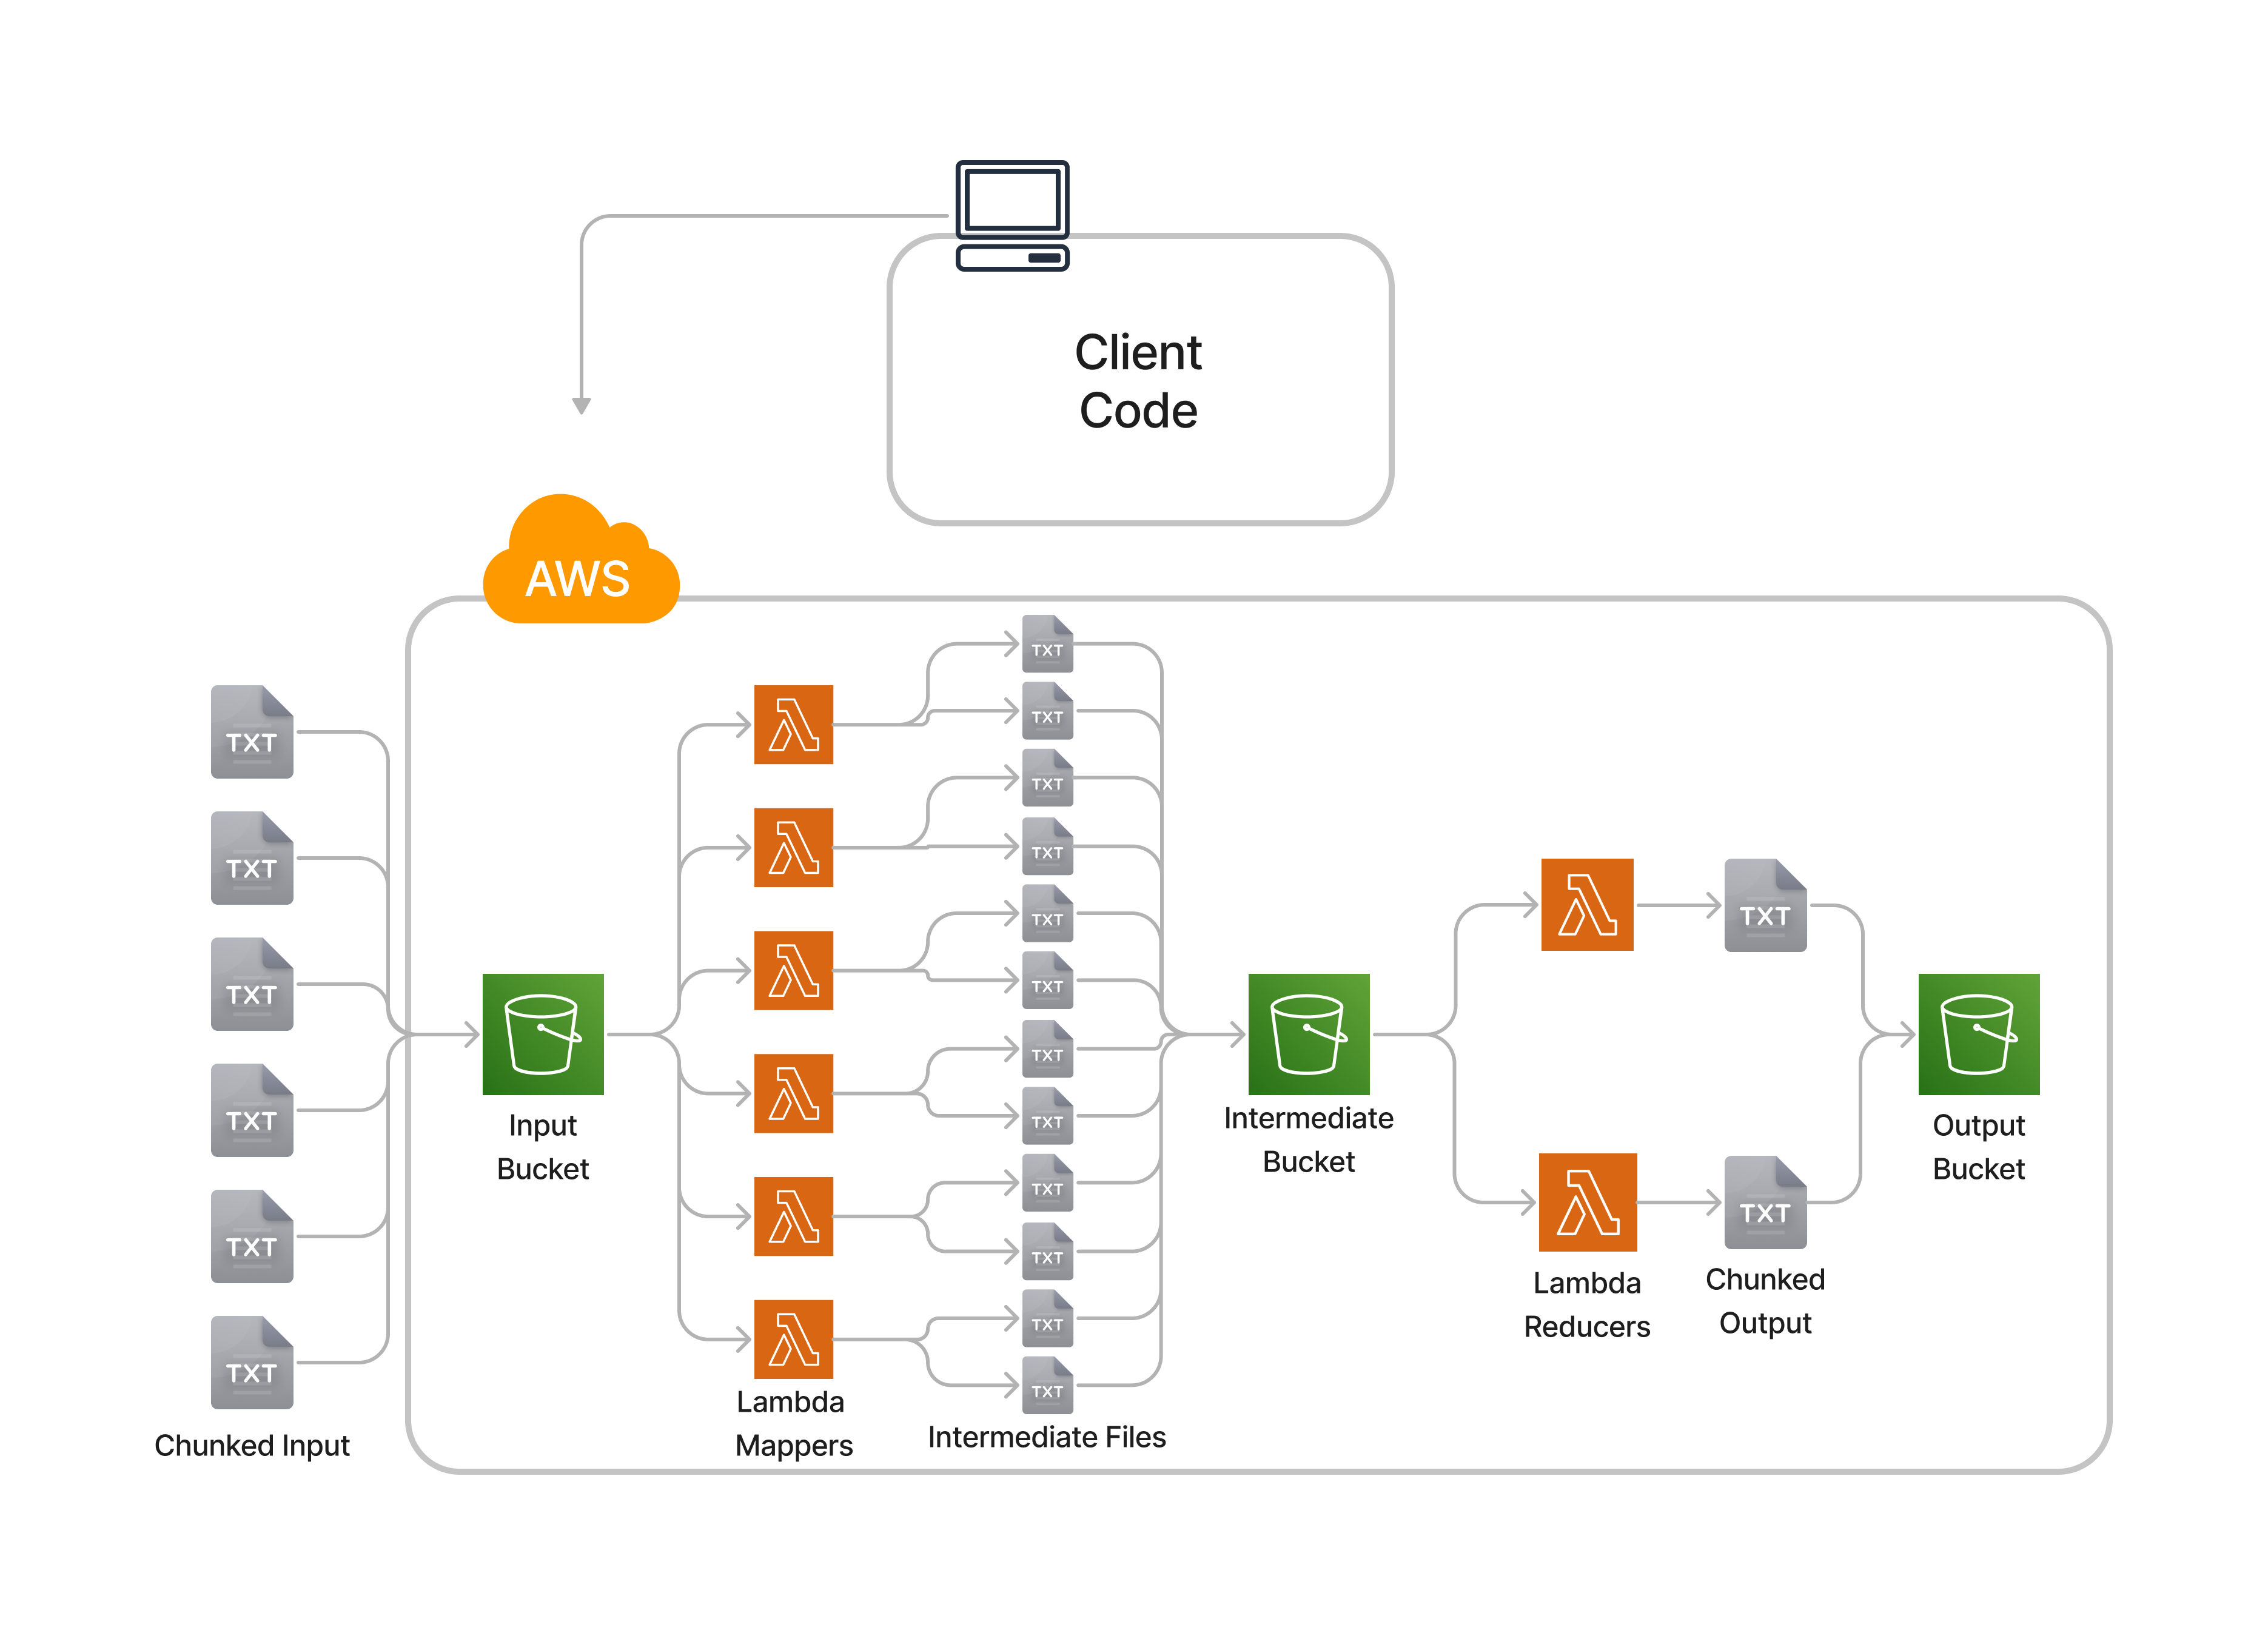
\includegraphics[width=\textwidth]{project_latex_template/images/arch.png}
\captionof{Figure 1.}{\small{ Architecture of the Serverless MapReduce runtime}}
\label{fig:arch}
\end{figure*}

In this section, we describe the architecture of our serverless MapReduce runtime and its functioning. The entire application consists of various parts like the client-side code, AWS S3 buckets, AWS Lambda functions and their associated code, and ancillary scripts for evaluation and testing. All code is written in Python. A detailed overview of the architecture is shown in Figure 1, with six mappers and two reducers.

\subsection{Components}

In order to make a Serverful MapReduce implementation work, two main components are needed: machines (or "nodes") that run the map or reduce jobs and an underlying distributed file system for sharing data. Google's implementation of MapReduce used the Google File System~\cite{ghemawat2003google} as the distributed file system. In our implementation, we used AWS S3- Amazon's highly scalable object store- as our distributed file system. Instead of long-running servers that run map or reduce tasks, our Serverless implementation will use short-lived AWS Lambda functions. Just like any other MapReduce implementation, the user defines \emph{Map(Key, Value)} and \emph{Reduce(Key, Value List)} functions based on their specific task.

The Serverless MapReduce implementation is supported by the following main components:

\begin{itemize}
    \item \emph{Input Bucket}: The input bucket stores the input corpus chunked into many files. The number of mappers invoked (\emph{m}) is equal to the number of chunks the input is divided into. Since Lambda is built for concurrent executions, this allows us to scale our workloads in a massively parallel manner by chunking the input as much as possible, beyond what may be possible for a Serverful implementation.
    
    \item \emph{Lambda Mappers}: When a Lambda Mapper is invoked, it is passed the input file and the number of reducers (\emph{n}) defined by the client. The mapper calls the user-defined \emph{Map(Key, Value)} on the file contents to obtain the intermediate key-value pairs. The mapper bins the intermediate key-value pairs based on the equation:
    \[bucket = hash(key) \pmod{n}\]
    Each of the \emph{n} intermediate files is encoded as JSON and stored in the intermediate bucket.
    
    \item \emph{Intermediate Bucket}: Each Mapper Lambda emits \emph{n} intermediate files that contain JSON-encoded key-value pairs and are stored in the intermediate S3 bucket. The total number of intermediate files for a given MapReduce job is $m\times{n}$. The files follow the naming convention:
    \[\emph{ReducerID\_InputChunkUID.json}\]
    Here, $ReducerID \in [0,n-1]$ and $InputChunkUID$ is a unique identifier associated with each input chunk. This naming convention is used by the runtime to figure out what reducers can be run and the files that need to be assigned to each reducer.
    
    \item \emph{Lambda Reducers}: When a Reducer Lambda is invoked, it is passed a list of all the intermediate files it needs to read and the \emph{ReducerID}. After reading all the relevant JSON data, the reducer transforms the key-value pairs into (key, value list) format. That is, for each unique key, we have a list of all the values associated with that key. The user-defined \emph{Reduce(Key, Value list)} function is called for each unique key to obtain the final output, which is encoded as JSON.
    
    \item \emph{Output Bucket}: Each of the \emph{n} reducers writes one file to the output bucket. To obtain the aggregate output of the MapReduce job, all the output chunks may have to be combined. If the output is in key-value pair form, it may be used as the input for another MapReduce job.
    
    \item \emph{Serverless MapReduce Client}: The Serverless MapReduce Client is the application the user interacts with to submit their MapReduce job. The main parameters the user has to specify are the S3 input bucket that contains the chunked input files and the number of reducers desired (\emph{n}).

    \item \emph{Miscellaneous Components}: Other parts of the system include AWS IAM roles and permission policies that allow communication between the various AWS services and ancillary components for combining output bucket data and comparing it against known values to validate the system.
\end{itemize}

Each Lambda was allocated a memory of 256 MB, 512 MB storage, and a timeout of 2 minutes.

\subsection{Workflow}

A typical run of a Serverless MapReduce job looks as follows:

\begin{enumerate}
    \item The user specifies their input bucket and the number of reducers (\emph{n}) and runs the MapReduce client.
    \item The MapReduce client invokes a Mapper Lambda for each input chunk. This can potentially be thousands of mappers.
    \item The Mapper Lambda stores its intermediate files (containing intermediate key-value pairs) in the intermediate bucket.
    \item Depending on what intermediate files have been written to the intermediate bucket, the MapReduce client figures out if any Reducer Lambdas are ready to run and invokes them until all \emph{n} reducers have been invoked.
    \item Once all the reducers are done, the chunked output is stored in the output S3 bucket. At this point, the output may be aggregated or passed on to another MapReduce job.
\end{enumerate}

\section{Testing}

[\textbf{TODO}: We have tested the validity of our implementation and it produces correct results for the project Gutenberg dataset. We plan to benchmark the performance of our implementation and compare it to other MapReduce implementations.]
\section{Architecture}

\begin{figure*}[!t]
\centering
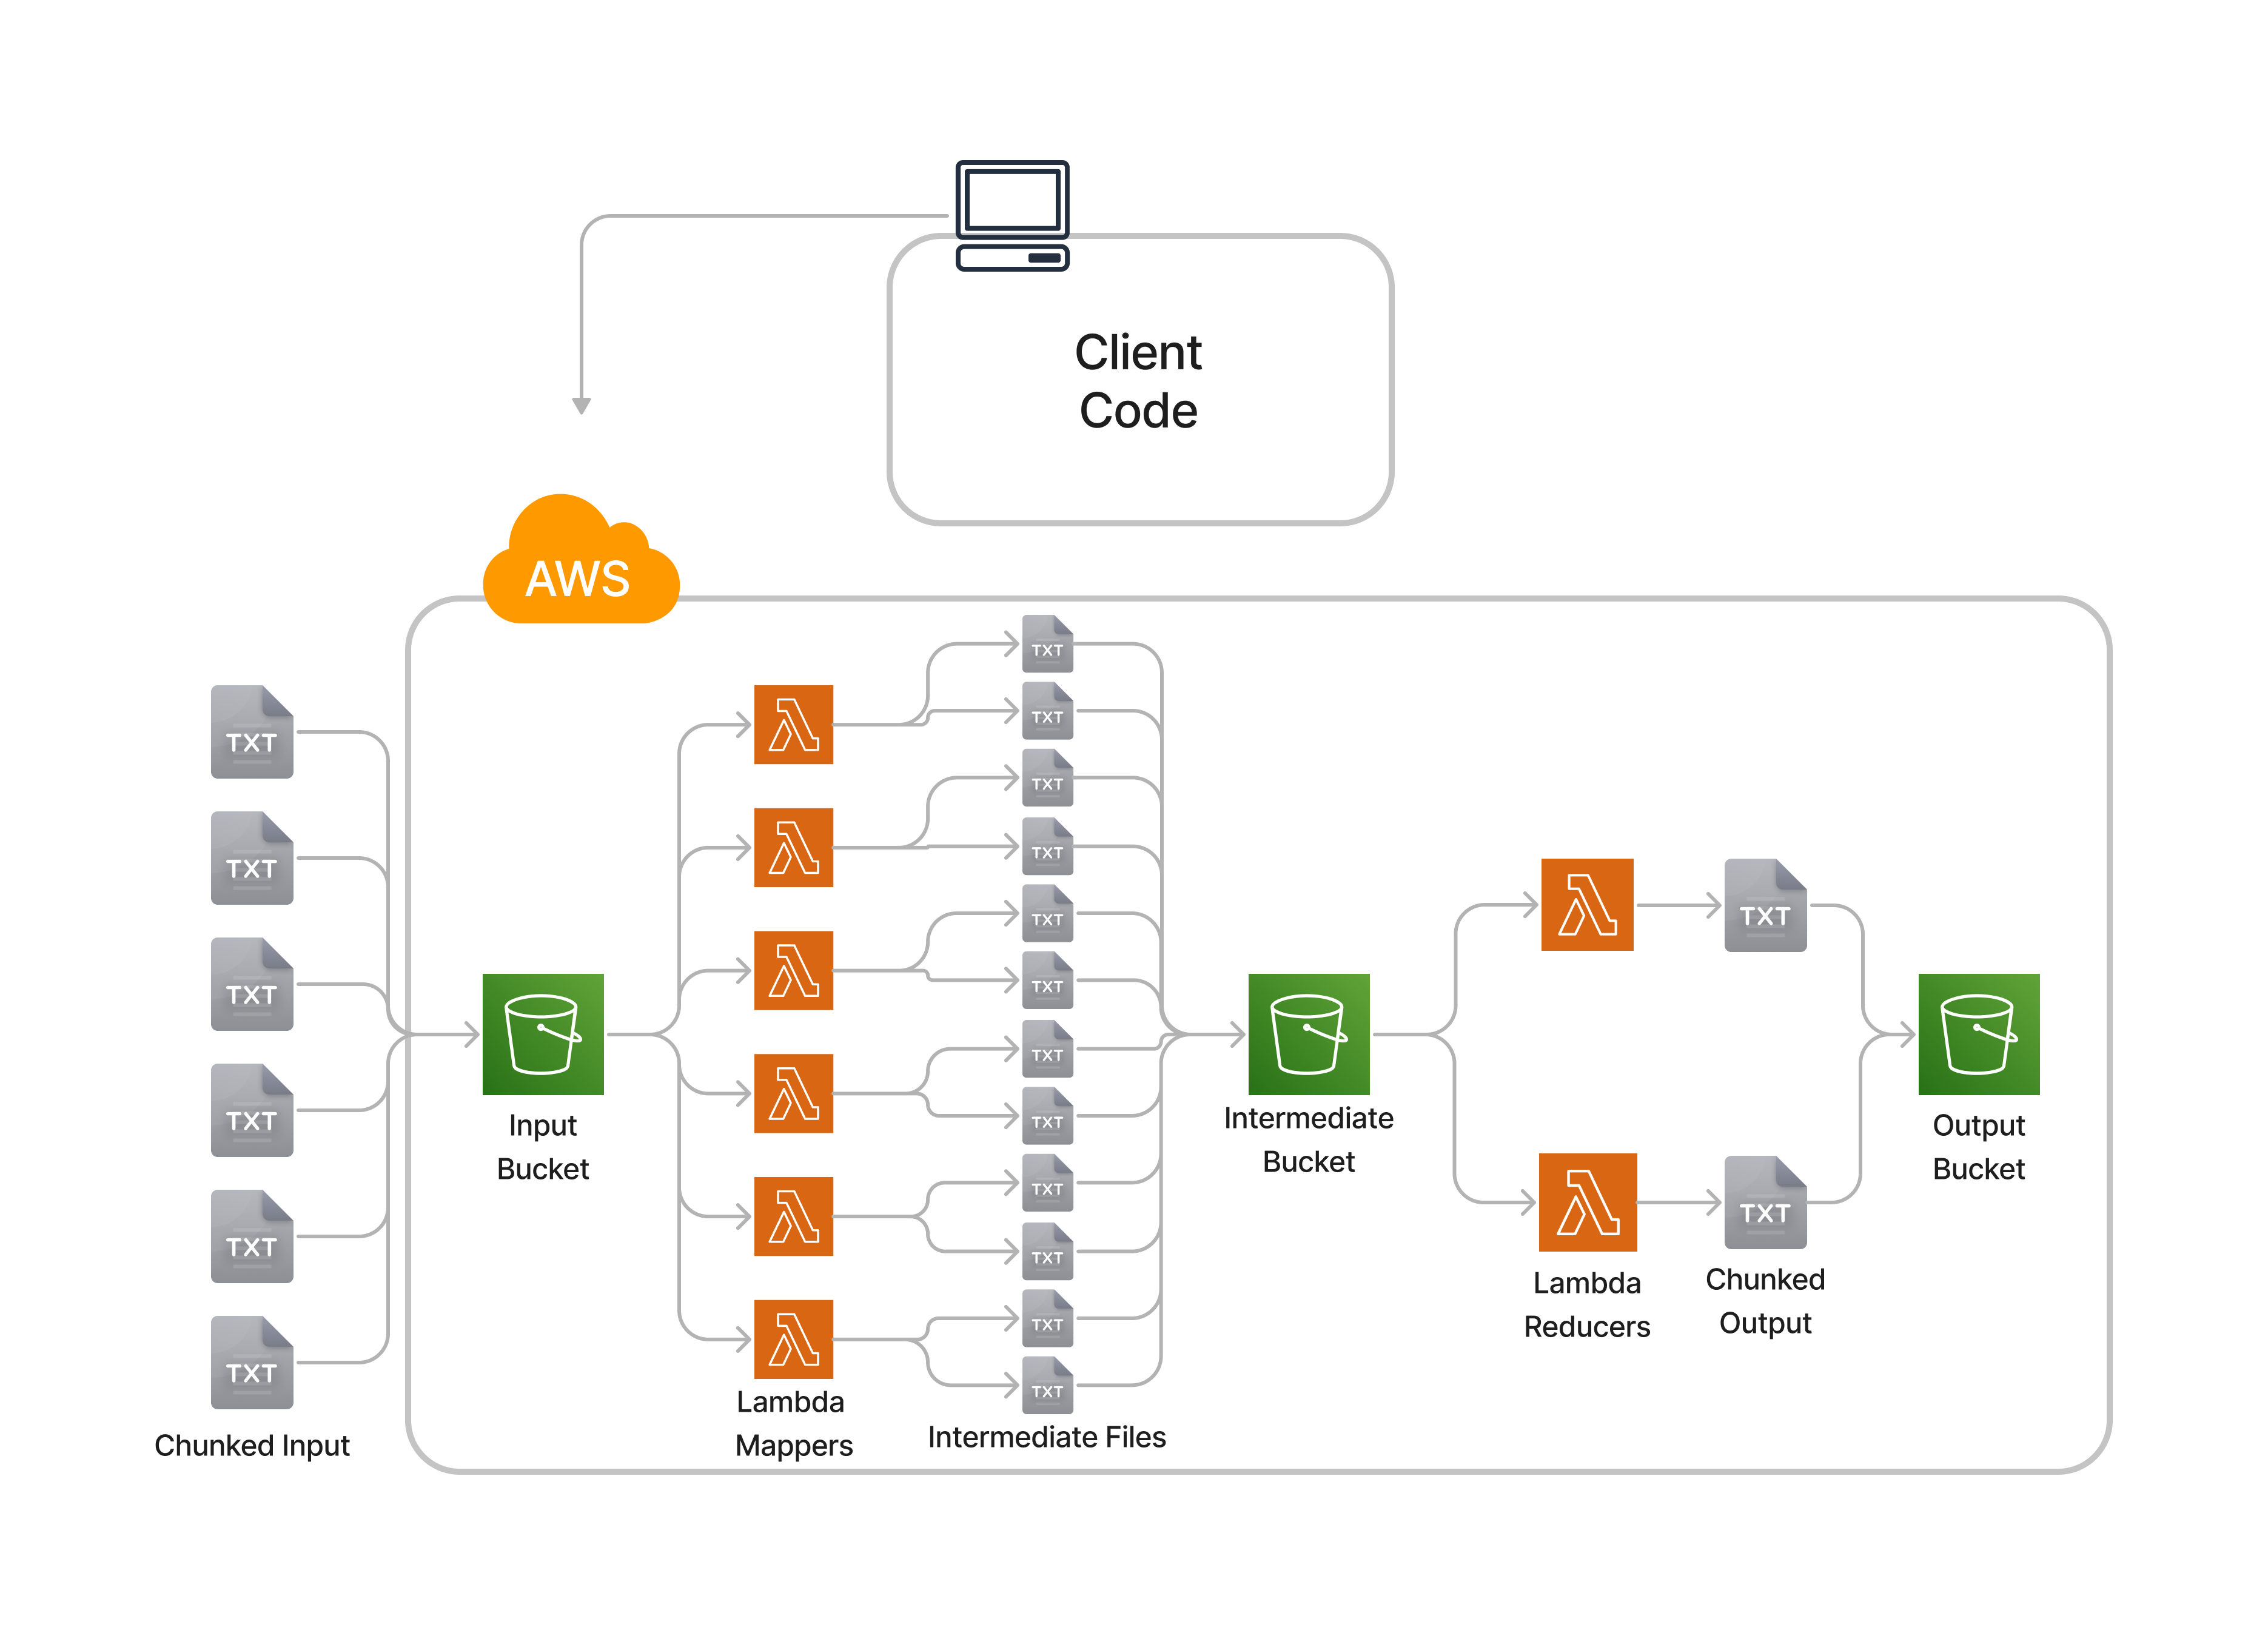
\includegraphics[width=\textwidth]{project_latex_template/images/arch.png}
\captionof{Figure 1.}{\small{ Architecture of the Serverless MapReduce runtime}}
\label{fig:arch}
\end{figure*}

In this section, we describe the architecture of our serverless MapReduce runtime and its functioning. The entire application consists of various parts like the client-side code, AWS S3 buckets, AWS Lambda functions and their associated code, and ancillary scripts for evaluation and testing. All code is written in Python. A detailed overview of the architecture is shown in Figure 1, with six mappers and two reducers.

\subsection{Components}

In order to make a Serverful MapReduce implementation work, two main components are needed: machines (or "nodes") that run the map or reduce jobs and an underlying distributed file system for sharing data. Google's implementation of MapReduce used the Google File System~\cite{ghemawat2003google} as the distributed file system. In our implementation, we used AWS S3- Amazon's highly scalable object store- as our distributed file system. Instead of long-running servers that run map or reduce tasks, our Serverless implementation will use short-lived AWS Lambda functions. Just like any other MapReduce implementation, the user defines \emph{Map(Key, Value)} and \emph{Reduce(Key, Value List)} functions based on their specific task.

The Serverless MapReduce implementation is supported by the following main components:

\begin{itemize}
    \item \emph{Input Bucket}: The input bucket stores the input corpus chunked into many files. The number of mappers invoked (\emph{m}) is equal to the number of chunks the input is divided into. Since Lambda is built for concurrent executions, this allows us to scale our workloads in a massively parallel manner by chunking the input as much as possible, beyond what may be possible for a Serverful implementation.
    
    \item \emph{Lambda Mappers}: When a Lambda Mapper is invoked, it is passed the input file and the number of reducers (\emph{n}) defined by the client. The mapper calls the user-defined \emph{Map(Key, Value)} on the file contents to obtain the intermediate key-value pairs. The mapper bins the intermediate key-value pairs based on the equation:
    \[bucket = hash(key) \pmod{n}\]
    Each of the \emph{n} intermediate files is encoded as JSON and stored in the intermediate bucket.
    
    \item \emph{Intermediate Bucket}: Each Mapper Lambda emits \emph{n} intermediate files that contain JSON-encoded key-value pairs and are stored in the intermediate S3 bucket. The total number of intermediate files for a given MapReduce job is $m\times{n}$. The files follow the naming convention:
    \[\emph{ReducerID\_InputChunkUID.json}\]
    Here, $ReducerID \in [0,n-1]$ and $InputChunkUID$ is a unique identifier associated with each input chunk. This naming convention is used by the runtime to figure out what reducers can be run and the files that need to be assigned to each reducer.
    
    \item \emph{Lambda Reducers}: When a Reducer Lambda is invoked, it is passed a list of all the intermediate files it needs to read and the \emph{ReducerID}. After reading all the relevant JSON data, the reducer transforms the key-value pairs into (key, value list) format. That is, for each unique key, we have a list of all the values associated with that key. The user-defined \emph{Reduce(Key, Value list)} function is called for each unique key to obtain the final output, which is encoded as JSON.
    
    \item \emph{Output Bucket}: Each of the \emph{n} reducers writes one file to the output bucket. To obtain the aggregate output of the MapReduce job, all the output chunks may have to be combined. If the output is in key-value pair form, it may be used as the input for another MapReduce job.
    
    \item \emph{Serverless MapReduce Client}: The Serverless MapReduce Client is the application the user interacts with to submit their MapReduce job. The main parameters the user has to specify are the S3 input bucket that contains the chunked input files and the number of reducers desired (\emph{n}).

    \item \emph{Miscellaneous Components}: Other parts of the system include AWS IAM roles and permission policies that allow communication between the various AWS services and ancillary components for combining output bucket data and comparing it against known values to validate the system.
\end{itemize}

Each Lambda was allocated a memory of 1,024 MB, 512 MB storage, and a timeout of 10 minutes.

\subsection{Workflow}

A typical run of a Serverless MapReduce job looks as follows:

\begin{enumerate}
    \item The user specifies their input bucket and the number of reducers (\emph{n}) and runs the MapReduce client.
    \item The MapReduce client invokes a Mapper Lambda for each input chunk. This can potentially be thousands of mappers.
    \item The Mapper Lambda stores its intermediate files (containing intermediate key-value pairs) in the intermediate bucket.
    \item Depending on what intermediate files have been written to the intermediate bucket, the MapReduce client figures out if any Reducer Lambdas are ready to run and invokes them until all \emph{n} reducers have been invoked.
    \item Once all the reducers are done, the chunked output is stored in the output S3 bucket. At this point, the output may be aggregated or passed on to another MapReduce job.
\end{enumerate}

% \begin{table*}[t]
% \centering
% \begin{tabular}{lllll}
% Test & Number of Files & Average File Size & Number of Mappers & Number of Reducers \\
%      &                 &                   &                   &                    \\
%      &                 &                   &                   &                    \\
%      &                 &                   &                   &                   
% \end{tabular}
% \end{table*}

\begin{table*}[h]
\centering
\begin{tabular}{|ccccccc|}
\hline
\multicolumn{7}{|c|}{Table I. Average Time to Complete MapReduce Jobs for Different Input Datasets}                                                                                                                                                                                                                                                                                                                                                                                                                                                               \\ \hline
\multicolumn{1}{|c|}{Test}   & \multicolumn{1}{c|}{\begin{tabular}[c]{@{}c@{}}Number \\ of Files\end{tabular}} & \multicolumn{1}{c|}{\begin{tabular}[c]{@{}c@{}}Average \\ File Size \\ (KB)\end{tabular}} & \multicolumn{1}{c|}{\begin{tabular}[c]{@{}c@{}}Total \\ Input Data \\ Size (MB)\end{tabular}} & \multicolumn{1}{c|}{\begin{tabular}[c]{@{}c@{}}Number \\ of Mappers\end{tabular}} & \multicolumn{1}{c|}{\begin{tabular}[c]{@{}c@{}}Number \\ of Reducers\end{tabular}} & \begin{tabular}[c]{@{}c@{}}Average Time \\ To Completion\\ (s)\end{tabular} \\ \hline
\multicolumn{1}{|c|}{Small}  & \multicolumn{1}{c|}{8}                                                          & \multicolumn{1}{c|}{412}                                                                  & \multicolumn{1}{c|}{3.3}                                                                      & \multicolumn{1}{c|}{8}                                                            & \multicolumn{1}{c|}{6}                                                             & 6.12                                                                        \\
\multicolumn{1}{|c|}{Medium} & \multicolumn{1}{c|}{98}                                                         & \multicolumn{1}{c|}{628}                                                                  & \multicolumn{1}{c|}{61.6}                                                                     & \multicolumn{1}{c|}{98}                                                           & \multicolumn{1}{c|}{80}                                                            & 26.44                                                                      \\
\multicolumn{1}{|c|}{Large}  & \multicolumn{1}{c|}{932}                                                        & \multicolumn{1}{c|}{687}                                                                  & \multicolumn{1}{c|}{644.1}                                                                    & \multicolumn{1}{c|}{932}                                                          & \multicolumn{1}{c|}{800}                                                           & 864.77                                                                     \\ \hline
\end{tabular}
\end{table*}

\section{Testing}

To evaluate the correctness of our MapReduce implementation and benchmark its performance, we decided to use the classic word count MapReduce task. We used books from the Project Gutenberg library to create input data sets of various sizes for our testing. The user-defined map and reduce functions for this task are presented below. This is the only thing the user has to specify in addition to the input files and number of reducers.

\begin{algorithm}
\caption{Map Function For Word Count}
\begin{algorithmic}[1]
\Function{UserMapFunction}{$k, v$}
    \State $words \gets [filtered~words~from~v]$
    \State $kv\_list \gets []$
    \For{$word$ \textbf{in} $words$}
        \State $kv\_list$.append(($word$.lower(), 1))
    \EndFor
    \State \Return $kv\_list$
\EndFunction
\end{algorithmic}
\end{algorithm}

\begin{algorithm}
\caption{Reduce Function For Word Count}
\begin{algorithmic}[2]
\Function{UserReduceFunction}{$k, \text{val\_list[]}$}
    \State \Return $\text{len}(\text{val\_list})$
\EndFunction
\end{algorithmic}
\end{algorithm}

\subsection{Methodology}

Using different books from the Project Gutenberg repository, we created test cases of increasing sizes. The number of Mapper Lambdas invoked is equal to the number of input files or chunks, and the number of Reducer Lambdas invoked is specified by the user. We created three total test cases: small, medium, and large. These scale from tens of Lambdas to about a thousand concurrently executing Lambda functions.

The different testing scenarios and their average completion times are presented in Table I. The current configurations allow 1,000 concurrent Lambda invocations, so some throttling was observed in the largest test case.

Each test scenario was run five times to obtain the average completion time across all runs. The number of reducers used was scaled appropriately based on how many input chunks each test scenario had. Making the number of reducers too small would result in Lambda invocations timing out as each reducer was overloaded with a lot more work, causing it to use up all its working memory and not finish before the timeout.

\subsection{Results}

The results in Table I demonstrate the highly scalable nature of implementing MapReduce on AWS Lambda and S3. The average job completion times we observed were small and scaled well as the size of the job increased. The smallest job took under 10 seconds to complete. The largest test case invokes almost 1,000 concurrently executing lambdas and writes 745,600 files to the intermediate bucket and 800 files to the output bucket. The total number of lambda invocations for the large test case is 1,732. The largest test case demonstrates the performance of our MapReduce runtime at scale. This test case was able to produce the result of the word count job in less than 15 minutes.

The main reason for the low average completion time, even in the largest case, is due to the massive parallelism that is allowed by concurrently executing Lambda functions. Also, S3 buckets provide rapid IO capabilities. In Section 5, we discuss methods to scale this even more in the future by increasing Lambda concurrency limits, and sub-dividing S3 buckets.

\section{Related Work}
\label{sec:related_work}

A similar project called MARLA~\cite{marla} to implement Serverless MapReduce was undertaken by the GRyCAP research group. The biggest difference between their architecture and ours is that they use a coordinator Lambda function that is triggered on an S3 bucket upload event. This coordinator Lambda is responsible for spawning Mappers, checking what Reducers are ready to run, the shuffle stage, and running the Reducers. In this architecture, the coordinator Lambda is likely to serve as a bottleneck for large jobs, as Lambda functions have a maximum runtime of 900 seconds and a maximum memory of 10,240 MB.

Another project called  Corral~\cite{corral} implements a similar architecture to what we have. It offers two ways to run the MapReduce job, either with a Coordinator Lambda function or using client-side code running locally on the user's machine. This implementation is written in Go and takes advantage of thread-level parallelism, which is not possible in a Python implementation. Due to this, it may offer faster performance overall for the coordinator's implementation.

\section{Conclusion}

[\textbf{TODO}: Draw conclusions about the feasibility of Serverless MapReduce based on the implementation process and the results obtained during the benchmarking.]


\section{Metadata}

\noindent
The code/data of the project can be found at:
\begin{center}
\fbox{\url{https://github.com/saarthak2002/serverless-mr}}
\end{center}



%-------------------------------------------------------------------------------
\bibliographystyle{plain}
\bibliography{ref}

\clearpage
\section*{Appendix A}
\begin{table}[h]
\centering
\begin{tabular}{|cccccccc|}
\hline
\multicolumn{8}{|c|}{Average S3 Storage Used And Lambda Runtime For Different Test Cases}                                                                                                                                                                                                                                                                                                                                                                                                                                                                                                                                                                                                                   \\ \hline
\multicolumn{1}{|c|}{Test} & \multicolumn{1}{c|}{\begin{tabular}[c]{@{}c@{}}Input\\ bucket\\ data size\end{tabular}} & \multicolumn{1}{c|}{\begin{tabular}[c]{@{}c@{}}Intermediate\\ bucket\\ data size\end{tabular}} & \multicolumn{1}{c|}{\begin{tabular}[c]{@{}c@{}}Output\\ bucket\\ data size\end{tabular}} & \multicolumn{1}{c|}{\begin{tabular}[c]{@{}c@{}}Number of\\ mapper lambda\\ invocations\end{tabular}} & \multicolumn{1}{c|}{\begin{tabular}[c]{@{}c@{}}Number of\\ reducer lambda\\ invocations\end{tabular}} & \multicolumn{1}{c|}{\begin{tabular}[c]{@{}c@{}}Avg runtime\\ of mapper \\ lambda\end{tabular}} & \begin{tabular}[c]{@{}c@{}}Avg runtime\\ of reducer\\ lambda\end{tabular} \\ \hline
Small                      & 3.3 MB                                                                                 & 7.7 MB                                                                                         & 528.1 KB                                                                                 & 8                                                                                                    & 6                                                                                                     & 26500                                                                                          & 20000                                                                     \\
Medium                     & 61.6 MB                                                                                & 120.2 MB                                                                                       & 7.4 MB                                                                                   & 98                                                                                                   & 80                                                                                                    & 37000                                                                                          & 27000                                                                     \\
Large                      & 644.1 MB                                                                               & 1100 MB                                                                                        & 156.7 MB                                                                                 & 932                                                                                                  & 800                                                                                                   & 37000                                                                                          & 27000                                                                     \\ \hline
\end{tabular}
\end{table}

%%%%%%%%%%%%%%%%%%%%%%%%%%%%%%%%%%%%%%%%%%%%%%%%%%%%%%%%%%%%%%%%%%%%%%%%%%%%%%%%
\end{document}
%%%%%%%%%%%%%%%%%%%%%%%%%%%%%%%%%%%%%%%%%%%%%%%%%%%%%%%%%%%%%%%%%%%%%%%%%%%%%%%%
